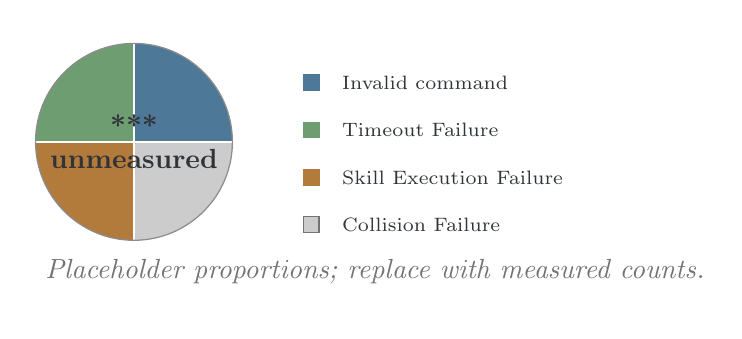
\begin{tikzpicture}[font=\rmfamily\fontsize{7.4}{8.2}\selectfont]
  \definecolor{piea}{HTML}{4D7898}
  \definecolor{pieb}{HTML}{6F9D72}
  \definecolor{piec}{HTML}{B27A3B}
  \definecolor{pietext}{HTML}{303438}
  \fill[piea] (0,0) -- (0:1.25) arc (0:90:1.25) -- cycle;
  \fill[pieb] (0,0) -- (90:1.25) arc (90:180:1.25) -- cycle;
  \fill[piec] (0,0) -- (180:1.25) arc (180:270:1.25) -- cycle;
  \fill[black!20] (0,0) -- (270:1.25) arc (270:360:1.25) -- cycle;
  \draw[white,line width=0.8pt] (0,0) -- (0:1.25);
  \draw[white,line width=0.8pt] (0,0) -- (90:1.25);
  \draw[white,line width=0.8pt] (0,0) -- (180:1.25);
  \draw[white,line width=0.8pt] (0,0) -- (270:1.25);
  \draw[black!45,line width=0.45pt] (0,0) circle (1.25);
  \node[font=\bfseries,text=pietext,align=center] at (0,0) {***\\unmeasured};
  \draw[piea,fill=piea] (2.15,0.65) rectangle (2.35,0.85);
  \node[anchor=west,text=pietext] at (2.52,0.75) {Invalid command};
  \draw[pieb,fill=pieb] (2.15,0.05) rectangle (2.35,0.25);
  \node[anchor=west,text=pietext] at (2.52,0.15) {Timeout Failure};
  \draw[piec,fill=piec] (2.15,-0.55) rectangle (2.35,-0.35);
  \node[anchor=west,text=pietext] at (2.52,-0.45) {Skill Execution Failure};
  \draw[black!55,fill=black!20] (2.15,-1.15) rectangle (2.35,-0.95);
  \node[anchor=west,text=pietext] at (2.52,-1.05) {Collision Failure};
  \node[anchor=west,text=black!55,font=\itshape] at (-1.25,-1.65)
    {Placeholder proportions; replace with measured counts.};
  \path[use as bounding box] (-1.35,-2.15) rectangle (5.95,1.45);
\end{tikzpicture}
